%\documentclass[a4paper]{article}
%\documentclass[sigconf]{acmart}
\documentclass{article}
\usepackage{nips_2018}

%\fancyhf{} % Remove fancy page headers 
%\fancyfoot[C]{\thepage}
%\setcopyright{none} % No copyright notice required for submissions
%\usepackage[small,compact]{titlesec}

\usepackage{enumitem}
%\settopmatter{printacmref=false, printccs=false, printfolios=true} % We want page numbers on submissions

%% Language and font encodings
\usepackage[english]{babel}
\usepackage[utf8x]{inputenc}
\usepackage[T1]{fontenc}

%% Sets page size and margins
%\usepackage[a4paper,top=1cm,bottom=1.5cm,left=2cm,right=2cm,marginparwidth=1.75cm]{geometry}

%% Useful packages
\usepackage{amsmath, amssymb, amsthm}
\usepackage{hyperref}
\usepackage{url}
\urlstyle{sf}
\usepackage{xcolor}
\usepackage{color}
\usepackage{balance}
% For figures
\usepackage{graphicx} % more modern
%\usepackage{epsfig} % less modern
\usepackage{subfigure} 
\usepackage{caption}
\usepackage{times}
\usepackage{natbib}
\usepackage{hyperref}
%\urlstyle{sf}
\usepackage{xcolor}
\usepackage{enumitem}
\usepackage{balance}
\usepackage{float}

\newcommand{\ak}[1]{\textcolor{blue}{\bf\small [#1 --Aleksandra]}}
\newcommand{\yd}[1]{\textcolor{violet}{\bf\small [#1 --Yatharth]}}
\newcommand{\todo}[1]{\textcolor{red}{TODO: {#1}}}
\newcommand\TODO[1]{\textcolor{red}{TODO: {#1}}}

\theoremstyle{plain}
\newtheorem{thm}{Theorem}[section]
\newtheorem{obs}{Observation}[section]
\newtheorem{lem}[thm]{Lemma}
\newtheorem{prop}[thm]{Proposition}
\newtheorem*{cor}{Corollary}
\newtheorem{defn}[thm]{Definition}

\title{The Power of The Hybrid Model for Mean Estimation}
%\author{Anonymized}

\begin{document}
\maketitle

\begin{abstract}
In this work we explore the power of the hybrid model of differential privacy (DP), as proposed in \cite{blender}. In particular, we study the accuracy of mean estimation algorithms for arbitrary distributions in bounded support. We show a hybrid mechanism that results from an optimally weighted convex combination of two sample mean estimates does a constant factor better for a wide range of sample sizes than natural benchmarks. We show how this improvement factor is parameterized by the problem setting and how it varies with sample size. 
\end{abstract}

\section{Introduction}

Differential privacy (DP), introduced by~\cite{dmns06}, has become the de facto standard of privacy in the computer science literature dealing with machine learning and statistical data analysis. Two traditional models of trust in the literature are the \textit{trusted curator model} and the \textit{local model}. In the trusted curator model, the analyst sees the true sample data and is able to calibrate noise to the sensitivity of the query. In the local model, the analyst is only able to access samples through some locally randomizing oracle. This means that each sample comes with noise calibrated to the sensitivity of the domain. Until recently, these models were employed mutually exclusively in practice. It is well understood theoretically and empirically that accuracy guarantees are far better in the trusted-curator model than in the local model \TODO{cite theoretical work, \cite{bittau2017prochlo}}. In practice, as discussed in more detail in \cite{blender}, it may often be the case that some small constant fraction of the samples trust the analyst while the rest require local randomization. In this case, the analyst has two natural options which we will use as benchmarks against which to compare the hybrid mechanism proposed here. First, the analyst could satisfy local DP for all of the samples. Second, the analyst could use only the opt-in samples and calibrate the noise appropriately. In this work, we consider how an analyst can improve their accuracy guarantees by running a query on each population and, satisfying exactly the privacy preferences of the two populations, outputting an optimal convex combination of the two query outputs.

In particular, we study the problem of mean estimation for arbitrary distributions in bounded support. We consider a hybrid mechanism that calculates a DP estimate of the mean of the opt-in samples (i.e., those who trust the analyst) and calculates the mean of the locally randomized samples and then outputs a convex combination of the two. The optimal weight for the convex combination depends on several parameters, such as the opt-in rate, total number of samples, the range of the support, and the privacy parameter. We compare this hybrid mechanism with the benchmarks outlined at the end of the previous paragraph \ak{weren't quite outlined, better to make concrete here than reference previous ones} \yd{what about now? should I still redefine the benchmarks, or is it more clear now?}. We characterize the outputs of these mechanisms as random variables and analyze the performance of our mechanisms using mean squared error.\footnote{We also explored the idea of comparing the performance of hybrid mechanism with alternatives in terms of their sample complexity, i.e., showing that the number of samples sufficient to get an accurate estimate with high probability in the hybrid model is less than the number of samples necessary to achieve the same for the benchmark mechanisms \ak{benchmark not defined}, but this proved difficult for several reasons. First, we found that the bound on the concentration of the sum of Laplace random variables in~\cite{Chan:2011:PCR:2043621.2043626} is nice to work with analytically, but is far from tight. In addition, the inherent lack of strength of the union bound limits what we can say about errors with several terms in their algebraic expressions. \ak{Example?} 

Another measure of performance we considered was absolute error. The trouble with this approach came from the difficulty in integrating one-sided probability density functions that arose from the convolution of several random variables, whether it was several Laplace random variables or a Laplace random variable and a Normal random variable. Finally, we decided that mean squared error was both comparatively straight-forward to calculate and, because of this, gave us a much more precise characterization of the performance of our mechanism against the benchmarks.}

\TODO{We find that, although the hybrid mechanism outperforms ... Need to write the conclusion of the work here!}
We find that the hybrid mechanism does in fact outperform the benchmarks. The improvement factor, while it depends on several problem parameters, is bounded roughly by 2. In \ref{sec:performance} we present analytical results describing this improvement factor in detail as well as empirical results showing the performance of the hybrid mechanism against the two benchmarks. 

\section{Models and Notation}
The data consists of data of $n$ individuals, where an individual $i \in [n]$ has data $x_i \in [0, m]$ drawn from distribution $\mathcal{D}$. The analyst only sees the original data of the $n_0 = c n$ individuals who opt in to the trusted curator model (TCM) of differential privacy. The rest of the $n_1 = (1-c) n$ individuals prefer the local model (LM) of differential privacy, where each individual randomizes their own data to satisfy $\epsilon$-DP and submits the noisy sample to the analyst. Note that $c$ is the opt-in rate, and naturally must be bounded such that $c \in [0,1]$. Further, we expect this $c$ to be small, as discussed in \ak{References for what a typical $c$ might be? Btw, we never mention that it is between 0 and 1}. In our analysis we will also refer to the variance of $\mathcal{D}$, which we will denote $\sigma^2$. The analyst would like to estimate the sample mean of the $n$ individuals such that each individual's trust preference is satisfied.

Assuming all $n$ samples are drawn from the same distribution $\mathcal{D}$, there are two ways to perform the estimate without hybridization. FullLM preserves local $\epsilon$-DP for all $n$ samples — each individual randomizes their own data using the Laplace mechanism before submitting it to the analyst. The analyst then calculates and outputs the mean of the noisy samples. \cite{duchi} and \cite{dky18} show that the Laplace mechanism is, in fact, optimal for the problem of one-dimensional mean estimation in the local model. The second mechanism, which we call OnlyTCM, uses only the $n_0$ opt-in samples to estimate the mean of all $n$ samples and perturbs the estimate using the Laplace mechanism.

We explore how much we can improve the accuracy of our estimate by using a hybrid mechanism, which we call Hybrid. This mechanism calculates two subsample means while preserving exactly the privacy preferences of each subsample. Hybrid runs OnlyTCM on the opt-in data and FullLM on the data that prefers local DP. It then outputs a convex combination of these two subsample means where the weight of the combination, which we will denote $w$, is computed to minimize the mean squared error of the estimate; this optimal weight will be denoted $w^*$. We will discuss precisely how $w^*$ is calculated in Lemma 4.3.

We use $\theta = \frac{1}{n}\sum_{i \in [n]}x_i$ to represent the true sample mean of all $n$ individuals. $\hat{\theta}$ will represent the analyst's $\epsilon$-DP estimate of the sample mean. We use $\theta_0 = \frac{1}{n_0}\sum_{i \in \{1, \dots, n_0\}} x_i$ to represent the true sample mean of the $n_0$ opt-in samples and $\hat{\theta}_0$ for the $\epsilon$-DP estimate of $\theta_0$ that satisfies TCM differential privacy. Note that $\hat{\theta}_0$ is obtained by running OnlyTCM on the data. Analogously, $\theta_1 = \frac{1}{n_1}\sum_{i \in \{n_0+1, \dots, n\}} x_i$ represents the true sample mean of the $n_1$ individuals who prefer LM differential privacy and $\hat{\theta}_1$ is the $\epsilon$-DP estimate of $\theta_1$ that satisfies LM differential privacy. Note that $\hat{\theta}_1$ is obtained by running FullLM on the $n_1$ samples that prefer local randomization. Hybrid returns the estimate
$\hat{\theta} = w^*\hat{\theta}_0 + (1-w^*)\hat{\theta}_1$.

\section{Preliminaries}
We derive expected squared errors using the moment generating functions (mgf) of the Laplace, Gaussian, and Normal-Laplace distributions. Thus in this section, we present the relevant functions and derive the second moment about the origin for each. These expressions will then be used in calculating the expected squared errors of the mechanisms of interest in Section~\ref{sec:performance}. 

\begin{lem}[2nd moment about origin, Laplace distribution]
Let $X \sim Lap(b)$. Then, $E[X^2] = 2b^2.$
\end{lem}
\begin{proof}
The moment generating function for $X$ is $M_X(t) = \frac{1}{1 - t^2b^2}.$
Then, $M''_X(t) = -\frac{2b^2(3b^2t^2 + 1)}{(b^2t^2 - 1)^3}.$
Plugging in $t = 0$, we get 
$E[X^2] = M''_X(0) = -\frac{2b^2}{(-1)^3} = 2b^2.$
\end{proof}

The Normal random variables relevant for the work have $\mu = 0$, so we focus on the central moments of the Normal distribution.

\begin{lem}[2nd central moment about origin, Normal distribution~\cite{papoulis2002probability}]
Let $X \sim Nor(0, \sigma^2)$. Then,
$E[X^2] = \sigma^2.$
\end{lem}

We will also need to consider the error of the sum of a Laplace random variable and a Normal random variable. %Thus, characterizing the distribution of such a random variable will prove essential.
\begin{defn}[Normal-Laplace distribution~\cite{Reed2006}]
A random variable $Y \overset{d}{=} Z + W,$ where $Z \sim Nor(\mu, \sigma^2)$ and $W \sim Lap(b)$, is distributed according to the Normal-Laplace distribution, which we denote $Y \sim NL(\mu, \sigma^2, b)$.
\end{defn}

As we did with the Normal distribution above, we focus on central moments of the Normal-Laplace distribution.
\begin{lem}[2nd central moment about origin, Normal-Laplace distribution]
\label{nl_secmom}
Let $X \sim NL(0, \sigma^2, b)$. Then, 
$E[X^2] = \sigma^2 + 2b^2.$
\end{lem}
\begin{proof}
The moment generating function for $X$ is
$M_X(t) = \frac{\exp(\sigma^2t^2/2)}{1 - b^2t^2}.$
Then, as the lemma states
$E[X^2] = M''_X(0) = \sigma^2 + 2b^2.$
\end{proof}

We will also need the following property of the Laplace distribution. 
\begin{lem} \label{wtimeslap}
Let $X \sim Lap(b)$ and $Y = wX$ where $w \in [0,1]$ is a constant. Then, 
$Y \sim Lap(wb).$
\end{lem}
\begin{proof}
Let $F_X$ be the cumulative distribution function (cdf) of $X$ and $f_X$ be the probability density function (pdf) of $X$. Let $F_Y$ and $f_Y$ be the same for $Y$. Then, by definition we have 
$F_Y(y) = Pr[Y \leq y] = Pr[X \leq y/w] = F_X(y/w).$
	
Evaluating the cdf of the Laplace distribution at $y/w$, we get 
$F_X(y/w) = 
	\begin{cases} 
      \frac{1}{2}e^{\frac{y}{bw}} & y < 0 \\
      1 - \frac{1}{2}e^{-\frac{y}{bw}} & y \geq 0 
	\end{cases} .$
	
Finally, we translate the cdfs to pdfs and the lemma follows immediately, \\
$f_Y(b) = \frac{d}{dy}F_Y(y) = \frac{d}{dy}F_X(y/w) $
$= \frac{1}{2bw}
	\begin{cases} 
      e^{\frac{y}{bw}} & y < 0 \\
      e^{-\frac{y}{bw}} & y \geq 0 
	\end{cases}
     = f_X(wb).$
\end{proof}



\section{Performance of Hybrid Mechanism}\label{sec:performance}
In this section we study the hybrid mechanism and the accuracy improvement it provides over the benchmarks, OnlyTCM and FullLM. We study the accuracy of these mechanisms by modeling their errors as random variables and studying their expectations, in particular, their second moments about the origin.

\begin{lem}[Expected squared error of FullLM]
\label{MSE_FullLM}
FullLM has expected squared error
$E[(\hat{\theta} - \theta)^2] = \frac{2m^2}{n\epsilon^2}.$
\end{lem}
\begin{proof}
FullLM returns estimate $\hat{\theta} = \theta + Z/n$ where $Z$ is the sum of $n$ random variables distributed according to $Lap(m/\epsilon)$. Then clearly, $\hat{\theta} - \theta = Z/n$ and therefore, by the Central Limit Theorem, $Z \sim Nor(0, 2nm^2/\epsilon^2)$ and the lemma follows. 
\end{proof}

\begin{lem}[Expected squared error of OnlyTCM]
\label{MSE_OnlyTCM}
OnlyTCM has expected squared error
$E[(\hat{\theta} - \theta)^2] = \frac{1}{cn}\left((1-c)\sigma^2 + \frac{2m^2}{cn \epsilon^2 }\right).$
\end{lem}
\begin{proof}
OnlyTCM returns the estimate $\hat{\theta} = \hat{\theta}_0$. Then we would like to study the following decomposition of the error
$\hat{\theta} - \theta = (\hat{\theta}_0 - \theta_0) + (1-c)(\theta_0 - \theta_1).$

The first term is a Laplace random variable
$\hat{\theta}_0 - \theta_0 \sim Lap\left(\frac{m}{cn\epsilon}\right).$

The second term is the difference of two sample means, so by Central Limit Theorem and the difference of Normally distributed random variables
$(1-c)(\theta_0 - \theta_1) \sim Nor\left(0, \frac{(1-c)\sigma^2}{cn}\right).$

Therefore, our error follows a Normal-Laplace distribution
$\hat{\theta} - \theta \sim NL\left(0, \frac{(1-c)\sigma^2}{cn}, \frac{m}{cn\epsilon} \right).$
Thus, the conclusion follows from Lemma~\ref{nl_secmom}.
\end{proof}

\begin{lem}[Expected squared error of Hybrid]
Hybrid has expected squared error 
$E[(\hat{\theta} - \theta)^2] = \frac{1}{(1-c)n}\left(\frac{(w^*-c)^2\sigma^2}{c} + \frac{2(1-w^*)^2 m^2}{\epsilon^2}\right) + \frac{2m^2w^{*2}}{c^2n^2\epsilon^2}$
where
$w^* = \frac{\frac{4 m^2}{(1-c) \epsilon^2 n}+\frac{2 \sigma^2}{(1-c) n}}{\frac{4 m^2}{c^2 \epsilon^2 n^2}+\frac{4 m^2}{(1-c) \epsilon^2 n}+\frac{2 \sigma^2}{(1-c) c n}}$
\end{lem}

\begin{proof}
We prove the optimality of $w^*$ at the end of this proof. For now, we study the distribution of the following decomposition of the error
$\hat{\theta} - \theta = w(\hat{\theta}_0 - \theta_0) + (1-w)(\hat{\theta}_1 - \theta_1) + (w-c)(\theta_0 - \theta_1).$

Notice that each of the terms in the above equation follow familiar distributions. In particular, the first term is simply a weight times the Laplace noise we add to the sample mean of the opt-in data. So, by Lemma \ref{wtimeslap},
$w(\hat{\theta}_0 - \theta_0) \sim Lap\left(\frac{wm}{cn\epsilon}\right).$

The second term is a weight times the sum of the Laplace noise that occurs from each local randomization. Then, by the Central Limit Theorem,
$(1-w)(\hat{\theta}_1 - \theta_1) \sim Nor\left(0, \frac{2(1-w)^2 m^2}{(1-c)n\epsilon^2}\right).$

The third term is the difference of two sample means, therefore, by Central Limit Theorem and the difference of two Normally distributed random variables, 
$(w-c)(\theta_0 - \theta_1) \sim Nor\left(0, \frac{(w-c)^2\sigma^2}{(1-c)cn}\right).$

Putting these together, we see that our error is distributed according to the following instantiation of the Normal-Laplace distribution
$\hat{\theta} - \theta \sim NL\left(0, \frac{1}{(1-c)n}\left(\frac{(w-c)^2\sigma^2}{c} + \frac{2(1-w)^2 m^2}{\epsilon^2}\right), \frac{wm}{cn\epsilon}\right).$

Then, it is easy to see by first order optimality that $w^*$ minimizes $E[(\hat{\theta} - \theta)^2]$.
\end{proof}

We can now analyze the improvement afforded by the optimal naive Hybrid mechanism presented above. We compare to the best of the two benchmarks. This depends on several parameters because the accuracy of OnlyTCM and FullLM vary with the parameters as per Lemmas~\ref{MSE_FullLM} and~\ref{MSE_OnlyTCM}. 

\begin{thm}[Hybrid vs. Benchmarks]\label{thm:main}
Define $\mathcal{E}_{\text{FullLM}}$ to be $E[(\hat{\theta} - \theta)]$ where $\hat{\theta}$ is returned by FullLM and let $\mathcal{E}_{\text{OnlyTCM}}$, $\mathcal{E}_{\text{Hybrid}}$ be similarly defined.
Let 
$R = \frac{\min(\mathcal{E}_{\text{FullLM}}, \mathcal{E}_{\text{OnlyTCM}})}{\mathcal{E}_{\text{Hybrid}}}$.
Then, 
$R = \gamma \cdot \frac{\epsilon^2 n \left(2 m^2 \left(c^2 n-c+1\right)+c \epsilon^2 n \sigma^2\right)}{2 c \epsilon^2 m^2 \sigma^2 (-c n+n+1)+4 m^4}$
where 
$\gamma = \min \left(\frac{2 m^2}{\epsilon^2 n},\frac{2 m^2-(c-1) c \epsilon^2 n \sigma^2}{c^2 \epsilon^2 n^2}\right).$
\end{thm}
\ak{Missing proof!} \yd{The proof is just plugging in and algebra, what should be written for this?}

Let $c_{\text{critical}} = \frac{\epsilon^2 \sigma^2}{\epsilon^2 \sigma^2+2 m^2}$ and let $n_{\text{critical}} = \frac{2 m^2}{c^2 \epsilon^2 \sigma^2+2 c^2 m^2-c \epsilon^2 \sigma^2}.$ Then, if $c>c_{\text{critical}}$ and $n > n_{\text{critical}}$, OnlyTCM has a smaller error than FullLM. While $n \leq n_{\text{critical}}$, FullLM has smaller error than OnlyTCM and the factor of improvement ($R$) increases linearly with $n$. 

\begin{cor}
The maximum value of $R$ is achieved at $n_{\text{critical}}$ and is equal to $R_{\text{max}} = \frac{2 (2-c) m^2}{(c-1) \epsilon^2 \sigma^2+2 m^2}.$
\end{cor}

\ak{Can you elaborate further on Theorem 4.4. and Corollary implications, and write about the figures?}
Theorem~\ref{thm:main} and its corollary provide a lower bound for the potential improvement provided by the hybrid model. Note that this improvement factor is 

\begin{figure}[t]
%\centering
\begin{minipage}[t]{.49\textwidth}
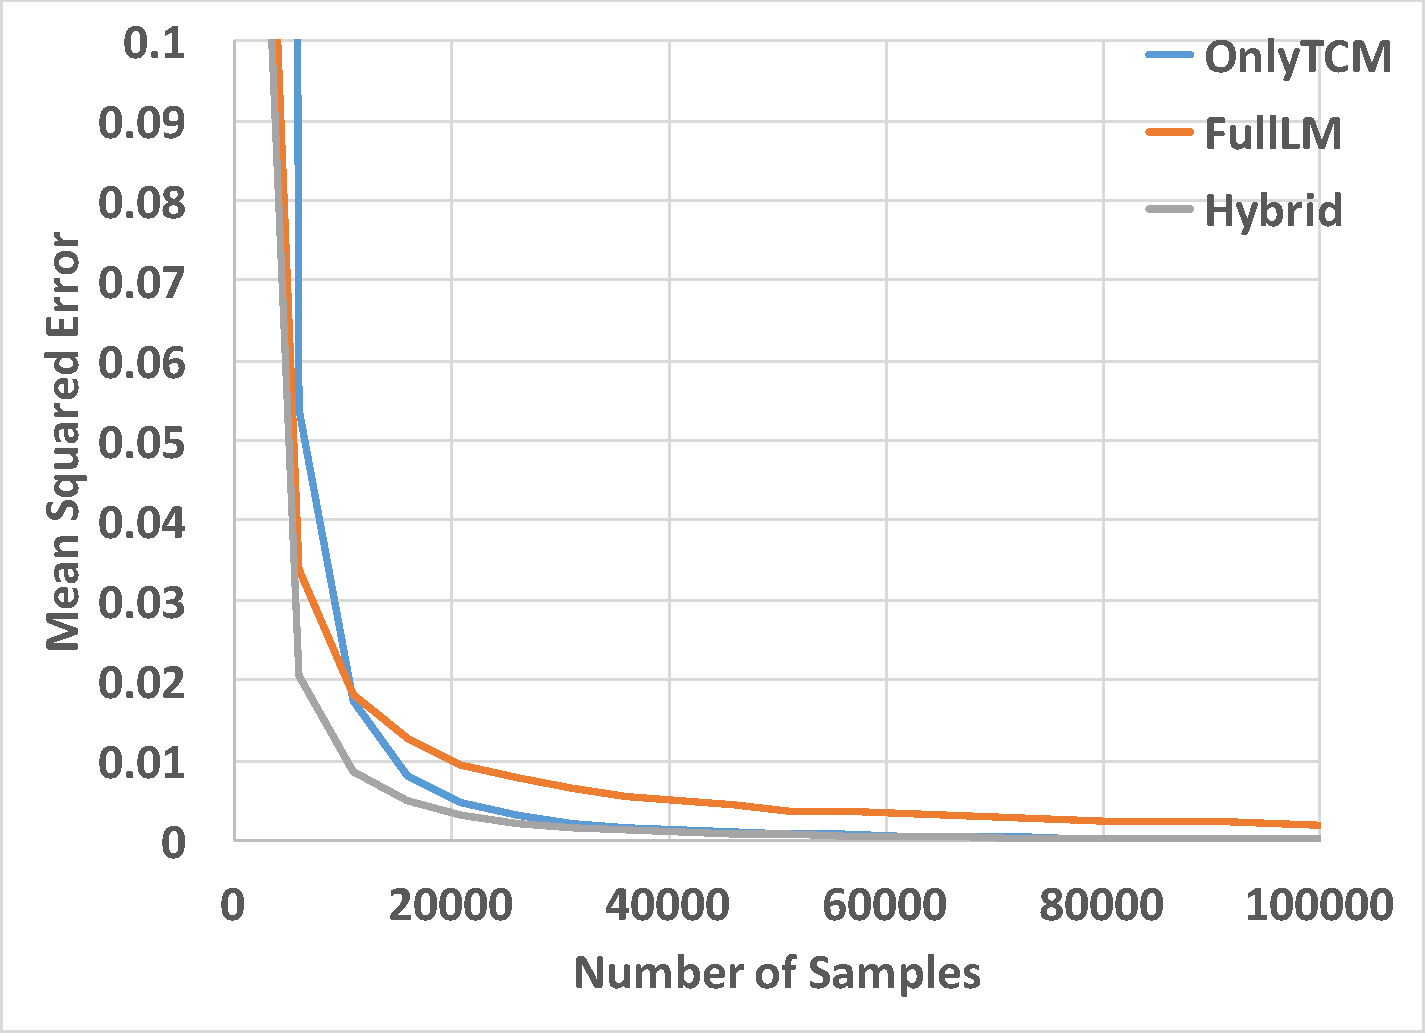
\includegraphics[width=0.99\linewidth]{eps01c01.pdf}
\caption{Relative performance of models for $c=0.01, \epsilon=0.1, m=1, \sigma = m/6$}
\end{minipage}
%\end{figure}
%\begin{figure}[t]
%\centering
\begin{minipage}[t]{.49\textwidth}
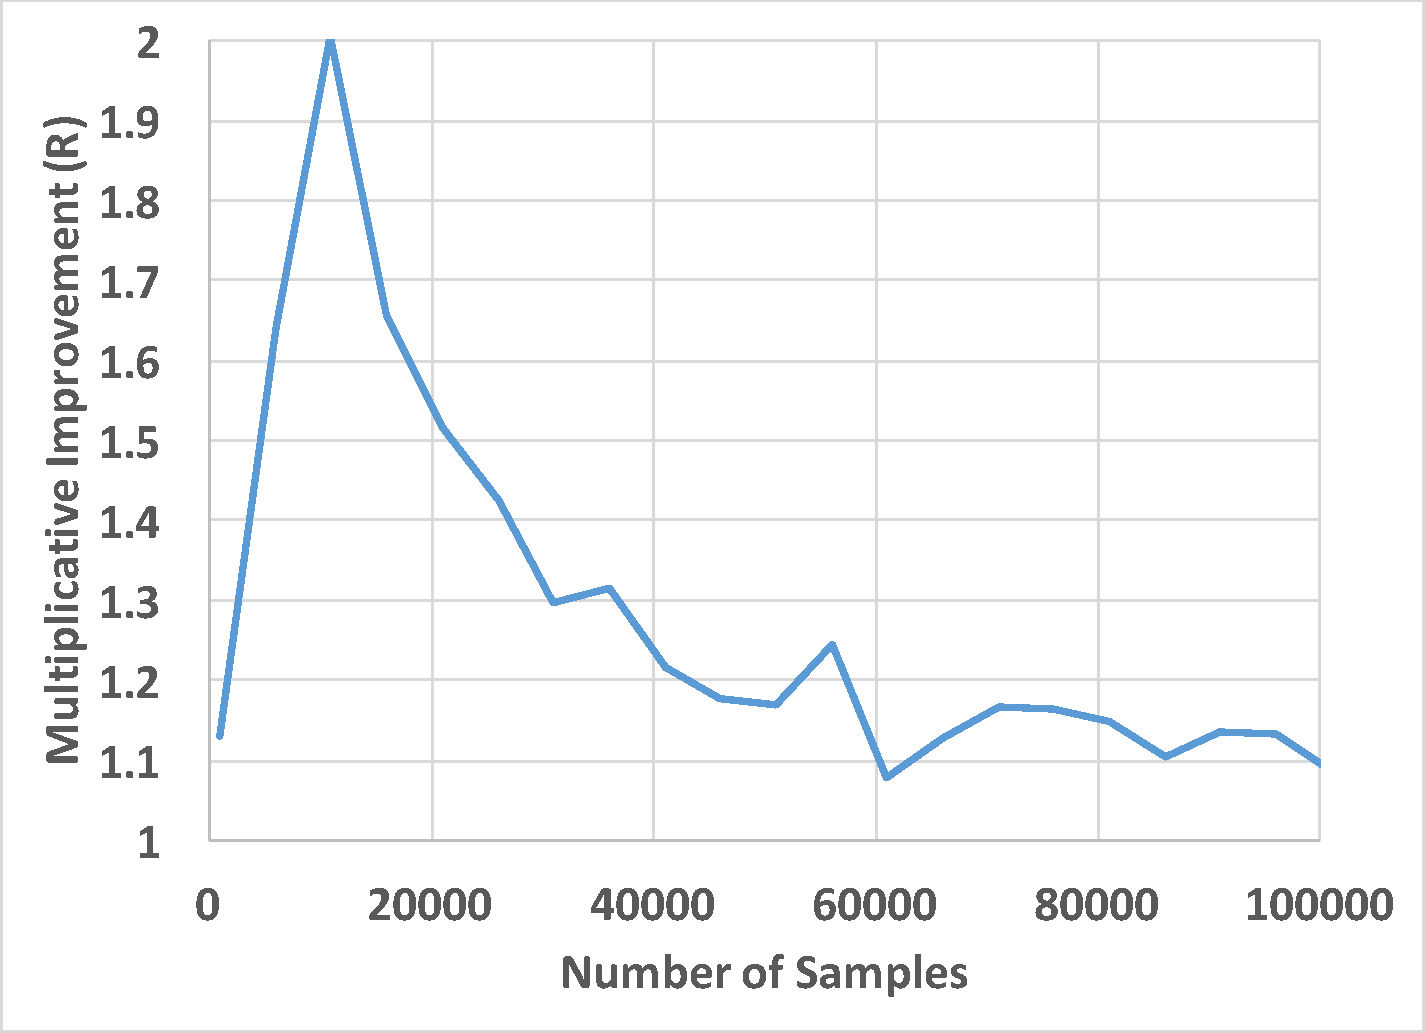
\includegraphics[width=0.99\linewidth]{imp_eps01c01.pdf}
\caption{Multiplicative improvement (R) given by Hybrid for $c=0.01, \epsilon=0.1, m=1, \sigma = m/6$}
\end{minipage}
\end{figure}

\section{Conclusions and Future Directions}
In this work, we looked at the accuracy of mean estimation algorithms in a hybrid trust environment. We propose a hybrid mechanism that calculates a DP estimate of the mean of the opt-in samples (i.e., those who trust the analyst) and calculates the mean of the locally randomized samples and then outputs a convex combination of the two. In particular, we showed that such a mechanism, where the weight of the convex combination is calculated to minimize mean squared error, can do a constant factor better for a large range of sample sizes, where the constant factor depends on several parameters.

Although for the problem of mean estimation, we were able to only do a constant factor better, we believe that there is more promise in considering hybrid mechanisms for more complex problems. \cite{Kasiviswanathan:2011:WLP:2078965.2078976} show that there exists separation between the class of problems that can be solved in the non-interactive local model and those that can be solved in the interactive local model. We conjecture that a hybrid mechanism that uses the opt-in samples to inform the local randomization can buy an increase in power similar to what is bought by interactivity. Therefore, a natural extension to our work is to show separation for hybrid DP and local DP. In particular, we would like to show that hybrid DP allows us to solve a natural variant of the masked parity problem from \cite{Kasiviswanathan:2011:WLP:2078965.2078976} that remains hard in the non-interactive local DP setting.

Perhaps a more tractable result would be to show that hybrid mechanisms perform better than the natural benchmarks for all counting queries. \cite{Blum:2005:PPS:1065167.1065184} show that counting queries are a powerful primitive that captures a large variety of machine learning and data-mining tasks, and therefore, showing that hybrid mechanisms can improve privacy-accuracy trade-offs for this class of queries and quantifying by how much would illustrate the power and limitations that can be gained by relying on a hybrid trust model. 

%\balance
\small
\bibliography{hybrid}
\bibliographystyle{alpha}
\end{document}